\documentclass{article}
%\usepackage[english]{babel}%
\usepackage{graphicx}
\usepackage{tabulary}
\usepackage{tabularx}
\usepackage[table,xcdraw]{xcolor}
\usepackage{pdflscape}
%\usepackage{gensymb}
\usepackage{lastpage}
\usepackage{multirow}
\usepackage{xcolor}
\usepackage{cancel}
\usepackage{amsmath}
\usepackage[table]{xcolor}
\usepackage{fixltx2e}
\usepackage[T1]{fontenc}
\usepackage[utf8]{inputenc}
\usepackage{ifthen}
\usepackage{fancyhdr}
\usepackage[utf8]{inputenc}
\usepackage{tikz}
\usepackage[document]{ragged2e}
\usepackage[margin=1in,top=1.2in,headheight=57pt,headsep=0.1in]
{geometry}
\usepackage{ifthen}
\usepackage{fancyhdr}
\everymath{\displaystyle}
\usepackage[document]{ragged2e}
\usepackage{fancyhdr}
\usepackage{mathabx}
\usepackage{textcomp,mathcomp}
\usepackage[shortlabels]{enumitem}
\everymath{\displaystyle}
\linespread{2}%controls the spacing between lines. Bigger fractions means crowded lines%
\linespread{1.3}%controls the spacing between lines. Bigger fractions means crowded lines%
\pagestyle{fancy}
\setlength{\headheight}{56.2pt}
\usepackage{soul}
\usepackage{siunitx}

%\usepackage{textcomp}
\usetikzlibrary{shapes.multipart, shapes.geometric, arrows}
\usetikzlibrary{calc, decorations.markings}
\usetikzlibrary{arrows.meta}
\usetikzlibrary{shapes,snakes}
\usetikzlibrary{quotes,angles, positioning}
%\chead{\ifthenelse{\value{page}=1}{\includegraphics[scale=0.3]{BassettCTCLogo}}}
%\rhead{\ifthenelse{\value{page}=1}{Final Exam}{}}
%\lhead{\ifthenelse{\value{page}=1}{Water Treatment - Oct-Dec 2022}{\textbf Final Exam}}
%\rfoot{\ifthenelse{\value{page}=1}{}{}}
%
%\cfoot{}
%\lfoot{Page \thepage\ of \pageref{LastPage}}
%\renewcommand{\headrulewidth}{2pt}
%\renewcommand{\footrulewidth}{1pt}
\begin{document}
\begin{enumerate}

\item What is the volume of water in ft$^3$, of a sedimentation basin that is 22 feet long, and 15 feet wide, and filled to 10 feet?

\item What is the volume in ft$^3$ of an elevated clear well that is 17.5 feet in diameter, and filled to 14 feet?

\item What is the area of the top of a storage tank that is 75 feet in diameter?\\

\item  What is the area of a wall $175 \mathrm{ft}$. in length and $20 \mathrm{ft}$. wide?\\

\item  You are tasked with filling an area with rock near some of your equipment. 1 Bag of rock covers 250 square feet. The area that needs rock cover is 400 feet in length and 30 feet wide. How many bags do you need to purchase?\\

\item A circular clearwell is 150 feet in diameter and 40 feet tall. The Clearwell has an overflow at 35 feet. What is the maximum amount of water the clearwell can hold in Million gallons rounded to the nearest hundredth?\\


\item  A sedimentation basin is 400 feet length, 50 feet in width, and 15 feet deep. What is the volume expressed in cubic feet?\\


\item  A clearwell holds $314,000 \mathrm{ft}^{3}$ of water. It is $100 \mathrm{ft}$ in diameter. What is the height of the clearwell?\\

\item  A treatment plant operator must fill a clearwell with $10,000 \mathrm{ft}^{3}$ of water in 90 minutes. What is the rate of flow expressed in GPM?\\


\item  A water tank has a capacity of 6MG. It is currently half full. It will take 6 hours to fill. What is the flow rate of the pump?\\


\item  A clearwell with the capacity of $2.5 \mathrm{MG}$ is being filled after a maintenance period. The flow rate is 2,500 GPM. The operator begins filling at 7 AM. At what time will the clearwell be full?\\

\item The floor of a rectangular building is 20 feet long by 12 feet wide and the inside walls are 10 feet high. Find the total surface area of the inside walls of this building\\
Solution:\\
% \begin{center}
\begin{tikzpicture}
	%%% Edit the following coordinate to change the shape of your
	%%% cuboid
      
	%% Vanishing points for perspective handling
	\coordinate (P1) at (-7cm,1.5cm); % left vanishing point (To pick)
	\coordinate (P2) at (8cm,1.5cm); % right vanishing point (To pick)

	%% (A1) and (A2) defines the 2 central points of the cuboid
	\coordinate (A1) at (0em,0cm); % central top point (To pick)
	\coordinate (A2) at (0em,-2cm); % central bottom point (To pick)

	%% (A3) to (A8) are computed given a unique parameter (or 2) .8
	% You can vary .8 from 0 to 1 to change perspective on left side
	\coordinate (A3) at ($(P1)!.8!(A2)$); % To pick for perspective 
	\coordinate (A4) at ($(P1)!.8!(A1)$);

	% You can vary .8 from 0 to 1 to change perspective on right side
	\coordinate (A7) at ($(P2)!.7!(A2)$);
	\coordinate (A8) at ($(P2)!.7!(A1)$);

	%% Automatically compute the last 2 points with intersections
	\coordinate (A5) at
	  (intersection cs: first line={(A8) -- (P1)},
			    second line={(A4) -- (P2)});
	\coordinate (A6) at
	  (intersection cs: first line={(A7) -- (P1)}, 
			    second line={(A3) -- (P2)});

	%%% Depending of what you want to display, you can comment/edit
	%%% the following lines

	%% Possibly draw back faces

	\fill[gray!40] (A2) -- (A3) -- (A6) -- (A7) -- cycle; % face 6
	\node at (barycentric cs:A2=1,A3=1,A6=1,A7=1) {\tiny Floor=W*L};
	
	\fill[gray!50] (A3) -- (A4) -- (A5) -- (A6) -- cycle; % face 3
	\node at (barycentric cs:A3=1,A4=1,A5=1,A6=1) {\tiny Wall - W*H};
	
	\fill[gray!10, opacity=0.2] (A5) -- (A6) -- (A7) -- (A8) -- cycle; % face 4
	\node at (barycentric cs:A5=1,A6=1,A7=1,A8=1) {\tiny Wall - L*H};
	
	\fill[gray!10,opacity=0.5] (A1) -- (A2) -- (A3) -- (A4) -- cycle; % f2
	\node at (barycentric cs:A1=1,A2=1,A3=1,A4=1) {\tiny Wall - L*H};
	
	\fill[gray!40,opacity=0.2] (A1) -- (A4) -- (A5) -- (A8) -- cycle; % f5
	\node at (barycentric cs:A1=1,A4=1,A5=1,A8=1) {\tiny Ceiling=W*L};	
	
	\draw[thick,dashed] (A5) -- (A6);
	\draw[thick,dashed] (A3) -- (A6);
	\draw[thick,dashed] (A7) -- (A6);

	%% Possibly draw front faces

	%\fill[orange] (A1) -- (A8) -- (A7) -- (A2) -- cycle; % face 1
	\node at (barycentric cs:A1=1,A8=1,A7=1,A2=1) {\tiny Wall - W*H};
	


	%% Possibly draw front lines
	\draw[thick] (A1) -- (A2);

	\draw[<->] (-1.8,0.38) -- (-1.8,-1.3)node [midway, above=-1.8mm] {\hspace{-1.3cm}\tiny Height=10'};
	\draw[<->] (-1.6,-1.4) -- (-.3,-2.1)node [midway, above=-2.6mm] {\hspace{-1.3cm}\tiny Length=20'};
	\draw[<->] (2.6,-1.13) -- (0.2,-2.2)node [midway, below=.6mm] {\hspace{1.2cm}\tiny Width=12'};
	\draw[thick] (A3) -- (A4);
	\draw[thick] (A7) -- (A8);
	\draw[thick] (A1) -- (A4);
	\draw[thick] (A1) -- (A8);
	\draw[thick] (A2) -- (A3);
	\draw[thick] (A2) -- (A7);
	\draw[thick] (A4) -- (A5);
	\draw[thick] (A8) -- (A5);
	
	% Possibly draw points
	% (it can help you understand the cuboid structure)
%	\foreach \i in {1,2,...,8}
%	{
%	  \draw[fill=black] (A\i) circle (0.15em)
%	    node[above right] {\tiny \i};
%	}
	% \draw[fill=black] (P1) circle (0.1em) node[below] {\tiny p1};
	% \draw[fill=black] (P2) circle (0.1em) node[below] {\tiny p2};
\end{tikzpicture}\\
% \end{center}
2 Walls W*H + 2 Walls L*H= $2*12*10ft^2 + 2*20*10ft^2$\\
$=240+400=\boxed{640ft^2}$\\

2 Walls W*H + 2 Walls L*H + Floor + Ceiling= $2*12*10ft^2 + 2*20*10ft^2 + 2*12*20ft^2$\\
$=240+400+480=\boxed{1,120ft^2}$\\

\item How many gallons of paint will be required to paint the inside walls of a 40 ft long x 65 ft wide x 20 ft high tank if the paint coverage is 150 sq. ft per gallon.  Note:  We are painting walls only.  Disregard the floor and roof areas.\\
Solution:\\
\vspace{0.3cm}
% \begin{center}
\begin{tikzpicture}
	%%% Edit the following coordinate to change the shape of your
	%%% cuboid
      
	%% Vanishing points for perspective handling
	\coordinate (P1) at (-7cm,1.5cm); % left vanishing point (To pick)
	\coordinate (P2) at (8cm,1.5cm); % right vanishing point (To pick)

	%% (A1) and (A2) defines the 2 central points of the cuboid
	\coordinate (A1) at (0em,0cm); % central top point (To pick)
	\coordinate (A2) at (0em,-2cm); % central bottom point (To pick)

	%% (A3) to (A8) are computed given a unique parameter (or 2) .8
	% You can vary .8 from 0 to 1 to change perspective on left side
	\coordinate (A3) at ($(P1)!.8!(A2)$); % To pick for perspective 
	\coordinate (A4) at ($(P1)!.8!(A1)$);

	% You can vary .8 from 0 to 1 to change perspective on right side
	\coordinate (A7) at ($(P2)!.7!(A2)$);
	\coordinate (A8) at ($(P2)!.7!(A1)$);

	%% Automatically compute the last 2 points with intersections
	\coordinate (A5) at
	  (intersection cs: first line={(A8) -- (P1)},
			    second line={(A4) -- (P2)});
	\coordinate (A6) at
	  (intersection cs: first line={(A7) -- (P1)}, 
			    second line={(A3) -- (P2)});

	%%% Depending of what you want to display, you can comment/edit
	%%% the following lines

	%% Possibly draw back faces

	\fill[gray!40] (A2) -- (A3) -- (A6) -- (A7) -- cycle; % face 6
	\node at (barycentric cs:A2=1,A3=1,A6=1,A7=1) {};
	
	\fill[gray!50] (A3) -- (A4) -- (A5) -- (A6) -- cycle; % face 3
	\node at (barycentric cs:A3=1,A4=1,A5=1,A6=1) {\tiny Wall - W*H};
	
	\fill[gray!10, opacity=0.2] (A5) -- (A6) -- (A7) -- (A8) -- cycle; % face 4
	\node at (barycentric cs:A5=1,A6=1,A7=1,A8=1) {\tiny Wall - L*H};
	
	\fill[gray!10,opacity=0.5] (A1) -- (A2) -- (A3) -- (A4) -- cycle; % f2
	\node at (barycentric cs:A1=1,A2=1,A3=1,A4=1) {\tiny Wall - L*H};
	
	\fill[gray!40,opacity=0.2] (A1) -- (A4) -- (A5) -- (A8) -- cycle; % f5
	\node at (barycentric cs:A1=1,A4=1,A5=1,A8=1) {};	
	
	\draw[thick,dashed] (A5) -- (A6);
	\draw[thick,dashed] (A3) -- (A6);
	\draw[thick,dashed] (A7) -- (A6);

	%% Possibly draw front faces

	%\fill[orange] (A1) -- (A8) -- (A7) -- (A2) -- cycle; % face 1
	\node at (barycentric cs:A1=1,A8=1,A7=1,A2=1) {\tiny Wall - W*H};
	


	%% Possibly draw front lines
	\draw[thick] (A1) -- (A2);

	\draw[<->] (-1.8,0.38) -- (-1.8,-1.3)node [midway, above=-1.8mm] {\hspace{-1.3cm}\tiny Height=20'};
	\draw[<->] (-1.6,-1.4) -- (-.3,-2.1)node [midway, above=-2.6mm] {\hspace{-1.3cm}\tiny Length=40'};
	\draw[<->] (2.6,-1.13) -- (0.2,-2.2)node [midway, below=.6mm] {\hspace{1.2cm}\tiny Width=65'};
	\draw[thick] (A3) -- (A4);
	\draw[thick] (A7) -- (A8);
	\draw[thick] (A1) -- (A4);
	\draw[thick] (A1) -- (A8);
	\draw[thick] (A2) -- (A3);
	\draw[thick] (A2) -- (A7);
	\draw[thick] (A4) -- (A5);
	\draw[thick] (A8) -- (A5);
	
	% Possibly draw points
	% (it can help you understand the cuboid structure)
%	\foreach \i in {1,2,...,8}
%	{
%	  \draw[fill=black] (A\i) circle (0.15em)
%	    node[above right] {\tiny \i};
%	}
	% \draw[fill=black] (P1) circle (0.1em) node[below] {\tiny p1};
	% \draw[fill=black] (P2) circle (0.1em) node[below] {\tiny p2};
\end{tikzpicture}\\
% \end{center}
\vspace{0.3cm}
2 Walls W*H + 2 Walls L*H = $2*65*20ft^2 + 2*40*20ft^2= 2,600+1,600=4,200ft^2$\\
$\implies @150\dfrac{ft^2}{gal} \enspace paint \enspace coverage \enspace \rightarrow \enspace \dfrac{4,200\cancel{ft^2}}{150\dfrac{\cancel{ft^2}}{gal}}=\boxed{28 \enspace gallons}$
\vspace{0.3cm}
\textbf{Example 3:}  What is the circumference of a 100 ft diameter circular sedimentation tank?\\
\vspace{0.3cm}
Solution:\\
\vspace{0.3cm}
$Circumference=\pi*D=3.14*100ft=\boxed{314ft}$
\vspace{0.3cm}

\textbf{Example 4:} If the surface area of a clarifier is 5,025$ft^2$, what is its diameter?\\
\vspace{0.3cm}
Solution:\\
\vspace{0.3cm}
$Surface \enspace area=\dfrac{\pi}{4}*D^2 \enspace \implies 5025(ft^2)=0.785*D^2 (ft^2)$\\
$\implies D^2=\dfrac{5025}{0.785} \implies D=\sqrt{6401.3}=\boxed{80ft}$
\vspace{0.3cm}

\item What is the surface area of a cylinder 80 ft diameter and 25 ft height?  Cylindrical part surface area only. Disregard the floor and roof areas.\\
*a.	6,280ft$^2$\\
b.	460ft$^2$\\
c.	25,425ft$^2$\\
d.	1,785ft$^2$\\
Solution:\\
\begin{center}
\begin{tikzpicture}[mydashed/.style={dashed,dash phase=2pt}]
\draw (0,0) ellipse (2cm and 0.3cm) node [midway, above=-2.4mm] {};
\draw (0,-2.3) ellipse (2cm and 0.3cm) node [midway, below=2.05cm] {};
\draw [-] (2,-2.3) -- (2,0);
%\draw [<->] (-2,0) -- (2,0); 
\draw [<->] (2.5,-2.3) -- (2.5,0) node [midway, below] {\hspace{2.9cm}Height (h) = 25'};
\draw [<->] (-2,-0.4) -- (2,-0.4) node [midway, below=0.7mm] {\hspace{0.1cm}\small{Diameter (D)}=80'};
%\draw [-] (0,-4) -- (2,-2.3);
%\draw [-] (0,-4) -- (-2,-2.3);
%\draw [-] (0,-4) -- (2,-2.3);
\draw [-] (-2,0) -- (-2,-2.3) node [midway, below] {\hspace{4cm}\tiny{Cylinder Surface Area$=\pi*D*h$}};
\draw [-latex, mydashed, line width=1mm, rotate=-90] (0.6,-1.9) arc [start angle=-120, end angle=120, x radius=0.8cm, y radius=2.2cm];
%\draw [-latex, thick, rotate=-95] (0,0) arc [start angle=-190, end angle=160, x radius=1cm, y radius=2cm];
\end{tikzpicture}\\

\end{center}
**************************************************************\\
1. Find the diameter of a settling basin that has a circumference of 126 feet.\\

2. Find the diameter of a pipe that has a circumference of 12 9/16".\\

Find the diameter of a storage tank that has a surface area of 314 ft2.\\

5. The detention time in a chlorine contact chamber is 42 minutes. If the chamber holds 3200 gallons, what is the flow rate in gpm?\\

6. A clearwell has a detention time of 2 hours. What is the flow rate in gpm if the
clearwell holds 8000 gallons?\\

7. A rectangular settling basin has a weir length of 10 feet. What is the weir overflow
rate when the flow is 80,000 gpd?\\

**************************************************************\\

$Surface \enspace area \enspace of \enspace cylinder=\pi*D*h=3.14*80*25=\boxed{6,280ft^2}$
\item How many gallons of water would 600 feet of 6-inch diameter pipe hold, approximately?\\
\vspace{0.3cm}
Solution:\\

\vspace{0.3cm}
% \begin{center}
\begin{tikzpicture}
\draw (0,0) ellipse (0.1cm and 0.3cm);
\draw (10,0) ellipse (0.1cm and 0.3cm);
\draw [-] (0,-0.29) -- (10,-0.29);
\draw [-] (0,0.29) -- (10,0.29);
\draw [<->] (10,-0.28) -- (10,0.28) node [midway, below=-3mm] {\hspace{2.6cm}Diameter=6"};
\draw [<->] (0,-.68) -- (10,-.68)node [midway, below] {\hspace{0.9cm}Length=600'};
\end{tikzpicture}
% \end{center}
\vspace{0.3cm}
$Volume=\dfrac{\pi}{4}D^2*L=0.785*\Big(\dfrac{6}{12}\Big)^2*600\cancel{ft^3}*7.48\dfrac{gallons}{\cancel{ft^3}}=\boxed{881 \enspace gallons}$
\vspace{0.3cm}

\item  A 110 ft diameter cylindrical tank with a 12 ft deep cone is operated at a side water depth of 20 ft.  Calculate the volume of water in the tank in $ft^3$.\\
Solution:\\
\begin{center}
\begin{tikzpicture}
\draw (0,0) ellipse (2cm and 0.3cm);
\draw (0,-2.3) ellipse (2cm and 0.3cm);
\draw (0,-.8) ellipse (2cm and 0.3cm);
\draw [-] (2,-2.3) -- (2,0);
\draw [<->] (-2,0) -- (2,0) node [midway, below=-0.9cm] {\hspace{0.9cm}Diameter (D)=110'}; 
\draw [<->] (-2.6,-2.3) -- (-2.6,0) node [midway, below=-.3cm] {\hspace{-2.6cm}Cylinder Height};
\draw [<->] (2.5,-2.3) -- (2.5,-0.8) node [midway, below=-0.2cm] {\hspace{5.2cm}Side Water Depth (SWD) =20'};
\draw [-] (0,-4) -- (2,-2.3);
\draw [-] (0,-4) -- (-2,-2.3);
\draw [-] (0,-4) -- (2,-2.3);
\draw [-] (-2,0) -- (-2,-2.3);
\draw [<->] (2.5,-2.3) -- (2.5,-4)node [midway, below=-0.4cm] {\hspace{3.8cm}Cone Depth (CD)=12'};
\end{tikzpicture}
\end{center}
$Digester \enspace volume=Volume_{cylinder}+Volume_{cone}$\\
$\implies Digester \enspace volume=\frac{\pi}{4}D^2*SWD+\frac{1}{3}*(\frac{\pi}{4}*D^2*CD)$\\
$=0.785*110^2*20+1.05*110^2*12=\boxed{227,988ft^3}$\\

\item A 150 ft diameter cylindrical tank with a 8 ft deep cone is operated at a side water depth of 12 ft.  Calculate the volume of water in the tank in MG.\\
Solution:\\
\begin{center}
\begin{tikzpicture}
\draw (0,0) ellipse (2cm and 0.3cm);
\draw (0,-2.3) ellipse (2cm and 0.3cm);
\draw (0,-.8) ellipse (2cm and 0.3cm);
\draw [-] (2,-2.3) -- (2,0);
\draw [<->] (-2,0) -- (2,0) node [midway, below=-0.9cm] {\hspace{0.9cm}Diameter (D)=150'}; 
\draw [<->] (-2.6,-2.3) -- (-2.6,0) node [midway, below=-.3cm] {\hspace{-2.6cm}Tank Height};
\draw [<->] (2.5,-2.3) -- (2.5,-0.8) node [midway, below=-0.2cm] {\hspace{5.2cm}Side Water Depth (SWD) =12'};
\draw [-] (0,-4) -- (2,-2.3);
\draw [-] (0,-4) -- (-2,-2.3);
\draw [-] (0,-4) -- (2,-2.3);
\draw [-] (-2,0) -- (-2,-2.3);
\draw [<->] (2.5,-2.3) -- (2.5,-4)node [midway, below=-0.4cm] {\hspace{3.8cm}Cone Depth (CD)=8'};
\end{tikzpicture}
\end{center}
$Tank \enspace volume=Volume_{cylinder}+Volume_{cone}$\\
\vspace{0.3cm}
$\implies Tank \enspace volume=\frac{\pi}{4}D^2*SWD+\frac{1}{3}*(\frac{\pi}{4}*D^2*CD)$\\
\vspace{0.3cm}
$=\Big[0.785*150^2*12+\dfrac{1}{3}*\dfrac{3.14}{4}*150^2*8\Big]ft^3*7.48\dfrac{gal}{ft^3}*\dfrac{MG}{1,000,000 \enspace gal}=\boxed{1.94MG}$\\


\item A sedimentation basin is 60 feet in diameter. What is the surface area of the tank?\\

 

\textbf{Solution:}

\vspace{0.2cm}

Surface Area=$\dfrac{\pi}{4}*\mathrm{D}^2=(0.785*(60 \enspace \mathrm{ft})^2 =\boxed{2,826 \mathrm{ft}^2}$

\item If a trench is $526 \mathrm{ft}$ long, $4.0 \mathrm{ft}$ wide, and $5.5 \mathrm{ft}$ deep, how many cubic yards of soil were excavated?\\
$$526 \times 4 \times 5.5=\frac{11,572 \mathrm{f}^{3}}{27}=428$$\\

\item Bow many gallons would be contained in a circular tank that is $100 \mathrm{ft}$. in diameter and $10 \mathrm{ft}$ deep?\\
a. $\quad 587,0.00$ gallons\\
b. 657,000 gallons\\
c. 1,340,000 gallons\\
d. $\quad 2,349,000$ gallons\\


\item In order to rebuild a manhole, it will be necessary to remove the asphalt from a 35-foot diameter circle in a street. The pavement area involved is:\\
a. $\quad 208 \mathrm{sq. ft}$\\
b. $\quad 241, \mathrm{sq. ft}$\\
c. $\quad 962 \mathrm{sq. ft}$\\
d. $\quad 1125 \mathrm{sq. ft}$\\

\item Calculate the area in square feet of: a space $100 \mathrm{ft}$ long and $75 \mathrm{ft}$ svide. $100 \times 75$ Ans. TTur Sq. Fr.\\

\item Calculate the volume of a rectangular tank 20 feet high, $100 \mathrm{ft}$ long, and 75 feet wike.\\
Ans. $\frac{10 \text { wo }}{1}$ Cu.Ft.\\

\item Calculate the gallons the tank in the preceding problem will hold. Ans. $1,122,000$ Gallons\\

\item Calculate the area in square feet of a space $40 \mathrm{ft}$ long and 50 feet vvide.\\
Ans, 2000 Sq. Ft\\

\item Calculate the volume of a rectangular tank 40 ft long, 50 ft wide and 25 feet tall.\\
$$\text { Ans. } 50,000 \text { Cu.Ft }$$\\

\item Calculate the gallons the tank in the preceding problem will contain.\\
Ans. 374,000 Gallons\\


\item Calculate the area of a circle with a $10 \mathrm{ft}$ radius.\\
Ans. $314 \quad$ Sq Ft\\

\item Calculate the aren of a circle with a 10 ft diameter.\\
Ans. $78-5$\\

\item Calculate the yolmue of a tank with a 50 ft diameter that is 20 feet high.\\
$$\text { Ans. } 39,260$$Cu. Ft\\

\item How many gallons will the tank in the preceding problem hold?\\

\item Calculate the area of a circle with a 100 ft dibmeter.\\
$$\text { Ans. } 293,590$$\\
Ans. $7,800 \mathrm{Sq} \mathrm{Ft}$\\

\item Calculate the volume of a tank with a $100 \mathrm{ft}$ diameter that is 50 feet high.\\
$$392,500$$\\
Ans.\\

\item How many gallons ryill the tank in the preceding problen hold? Auls.\\
$2,935,960$\\
$$18 \times 18 \times 0^{\prime} 0408 \times 1200$$\\

\item How many gallons will an $18^{\prime \prime}$ diameter pipeline, 1200 ' long contain?\\
$$\text { imi }=5280 \text { Ans. 15,863 Gallons }$$\\

\item How many gallons will a 24 " pipeline, 2 miles long contain?\\
$$24 \times 24 \times 0.0408 \times \quad 248,168$$\\



\item How many gallons will an $8^{\prime \prime}$ pipeline 550 ' long contain?\\
$$8 \times 8 \times 0.0408 \times 550$$\\
Ans. $1436 \cdot \frac{16}{\text { gallons }}$\\

\item Water is filling a tank at the rate of 50 gpm for a 10 min. period, How many gallons of water are contained in the tank at the end of the 10 minute time period?\\

\item A well pump is discharging water at the rate of 400 gpm into a tank for 15 minutes. Haw many gallons will be in the tank at the end of this time period?\\
$$6,000 \ldots \text { Gal. }$$\\
Dose $=$ Dewand T Resrdual $\frac{300}{20} \times 16$\\

\item A tank is filling at the rate of $300 \mathrm{gpm}$ for a 20 minute period. How many of water will be contained in the tank at the end of 16 minutes?\\
4880 Gal.\\


\item How many galtons will the above cylinder hold?\\
$100 \times 7.48=748$\\

\item Calculate the area in square feet of a space $100 \mathrm{ft}$. long and $75 \mathrm{ft}$ widie.\\
Ans. $7500 \quad$ Sq. Fit\\

\item Calculate the volume of a rectangular tank 20 feet high, $100 \mathrm{ft}$ long, and 75 feet wide.\\
Ans. $150,00 \quad$ Cu.F.\\

\item Calculate the gallons the tauk in the preceding problem will hold.\\

\item Calculate the area in square feet of a space $40 \mathrm{ft}$ long and 50 feet wide.\\
Ans, $\frac{2,000}{1}$ Sq. Ft\\

\item Calculate the volume of a rectangular tank $40 \mathrm{ft}$ long, $50 \mathrm{ft}$ wide and 25 feet tall.\\
Ans. $50000 \quad \mathrm{Cu} . \mathrm{Ft}$\\

\item Calculate the gallons the tank in the preceding problem will contain.\\
$$50,000 \times 7.48 \text { Ans. } 374,000 \text { Gallons }$$\\

\item Caiculate the area of a circle with a $10 \mathrm{ft}$ radius.\\
$$D=20 \text {. }$$\\
Ans. $314 \quad \mathrm{Sq} \mathrm{Ft}$\\

\item Calculate the area of a circle with a 10 ft diameter.\\
Ans. $78.5 \quad \mathrm{Sq} \mathrm{Ft}$\\

\item Calculate the volume of a tank with a $50 \mathrm{ft}$ diameter that is 20 feet high.\\
$$\text { Ans. } 250 \quad \mathrm{Cu} \text {. Ft }$$\\

\item How many gallons will the tank in the preceding problem hold?\\

\item Calculate the area of a circle with a $100 \mathrm{ft}$ ciameter.\\
Ans. $\frac{293590}{7850}$ Gallons\\

\item Caiculate the volume of a tank with a $100 \mathrm{ft}$ diameter that is 50 feet higl,\\
$$392,50$$\\
$\frac{300 \text { gallons }}{1 \text { mute }} \times 6 \mathrm{~mm}$\\

\item A tank is filling at the rate of $300 \mathrm{gpm}$ for a 20 minute period. How many of water will be contained in the tank at the end of 16 minutes?\\

\item What is the area of a circular tank pad in ft2, if it has a diameter of 102 ft?\\
a.	6,160 ft2\\
b.	6,167 ft2\\
c.	8,170 ft2\\
d.	8,200 ft2\\

\item A 60-foot diameter tank contains 422,000 gallons of water. Calculate the height of water in the storage tank.

Volume = Area * Height $\implies Height (ft) =\dfrac{Volume - \cancelto{ft}{ft^3}}{Area \cancel{ft^2}}$\\
\vspace{0.2cm}
\

$ Volume \enspace (ft^3) = \dfrac{\pi}{4}*D^2 * fill height = 0.785*17.5^2 \enspace ft^2 * 14 ft=\boxed{240\enspace ft^3}$


\item What is the volume of water in ft$^3$, of a sedimentation basin that is 22 feet long, and 15 feet wide, and filled to 10 feet?\\

Volume = Length * Width * Height = 22 ft * 15 ft * 10 ft = $\boxed{3300 \enspace ft^3}$\\
\vspace{0.2cm}
$ Volume \enspace (ft^3) = \dfrac{\pi}{4}*D^2 * fill \enspace height = 0.785*17.5^2 \enspace ft^2 * 14 ft=\boxed{240\enspace ft^3}$

\item What is the volume in ft$^3$ of an elevated clear well that is 17.5 feet in diameter, and filled to 14 feet?

Volume = Area * Height\\
\vspace{0.2cm}
$ Volume \enspace (ft^3) = \dfrac{\pi}{4}*D^2 * fill height = 0.785*17.5^2 \enspace ft^2 * 14 ft=\boxed{240\enspace ft^3}$

\item What is the area of the top of a storage tank that is 75 feet in diameter?\\

$Area \enspace (ft^2)= \dfrac{\pi}{4}*D^2= 0.785*75^2 \enspace ft^2=0.785 = \boxed{4416\enspace ft^2}$\\
\vspace{0.2cm}

\item  What is the area of a wall $175 \mathrm{ft}$. in length and $20 \mathrm{ft}$. wide?\\
\vspace{0.2cm}
Solution:\\
\vspace{0.2cm}
Area = $175 * 20 \enspace = \enspace \boxed{3,500 ft^2}$
\vspace{0.2cm}
\item  You are tasked with filling an area with rock near some of your equipment. 1 Bag of rock covers 250 square feet. The area that needs rock cover is 400 feet in length and 30 feet wide. How many bags do you need to purchase?\\

\vspace{0.2cm}
Solution:\\
\vspace{0.2cm}
Area to be covered = 400' * 30' = 12,000 $ft^2$
\vspace{0.2cm}
$\implies 12,000 \enspace \cancel{ft^2} \enspace * \dfrac{Bag}{250 \enspace \cancel{ft^2}}=\boxed{48 \enspace bags}$


\item How many gallons of paint will be required to paint the walls of a 40 ft long x 65 ft wide x 20 ft high tank if the paint coverage is 150 sq. ft per gallon.  Note:  We are painting walls only.  Disregard the floor and roof areas.\\
Solution:\\
\begin{center}
\begin{tikzpicture}
	%%% Edit the following coordinate to change the shape of your
	%%% cuboid
      
	%% Vanishing points for perspective handling
	\coordinate (P1) at (-7cm,1.5cm); % left vanishing point (To pick)
	\coordinate (P2) at (8cm,1.5cm); % right vanishing point (To pick)

	%% (A1) and (A2) defines the 2 central points of the cuboid
	\coordinate (A1) at (0em,0cm); % central top point (To pick)
	\coordinate (A2) at (0em,-2cm); % central bottom point (To pick)

	%% (A3) to (A8) are computed given a unique parameter (or 2) .8
	% You can vary .8 from 0 to 1 to change perspective on left side
	\coordinate (A3) at ($(P1)!.8!(A2)$); % To pick for perspective 
	\coordinate (A4) at ($(P1)!.8!(A1)$);

	% You can vary .8 from 0 to 1 to change perspective on right side
	\coordinate (A7) at ($(P2)!.7!(A2)$);
	\coordinate (A8) at ($(P2)!.7!(A1)$);

	%% Automatically compute the last 2 points with intersections
	\coordinate (A5) at
	  (intersection cs: first line={(A8) -- (P1)},
			    second line={(A4) -- (P2)});
	\coordinate (A6) at
	  (intersection cs: first line={(A7) -- (P1)}, 
			    second line={(A3) -- (P2)});

	%%% Depending of what you want to display, you can comment/edit
	%%% the following lines

	%% Possibly draw back faces

	\fill[gray!40] (A2) -- (A3) -- (A6) -- (A7) -- cycle; % face 6
	\node at (barycentric cs:A2=1,A3=1,A6=1,A7=1) {\tiny Floor};
	
	\fill[gray!50] (A3) -- (A4) -- (A5) -- (A6) -- cycle; % face 3
	\node at (barycentric cs:A3=1,A4=1,A5=1,A6=1) {\tiny Wall - W*H};
	
	\fill[gray!10, opacity=0.2] (A5) -- (A6) -- (A7) -- (A8) -- cycle; % face 4
	\node at (barycentric cs:A5=1,A6=1,A7=1,A8=1) {\tiny Wall - L*H};
	
	\fill[gray!10,opacity=0.5] (A1) -- (A2) -- (A3) -- (A4) -- cycle; % f2
	\node at (barycentric cs:A1=1,A2=1,A3=1,A4=1) {\tiny Wall - L*H};
	
	\fill[gray!40,opacity=0.2] (A1) -- (A4) -- (A5) -- (A8) -- cycle; % f5
	\node at (barycentric cs:A1=1,A4=1,A5=1,A8=1) {\tiny Ceiling};	
	
	\draw[thick,dashed] (A5) -- (A6);
	\draw[thick,dashed] (A3) -- (A6);
	\draw[thick,dashed] (A7) -- (A6);

	%% Possibly draw front faces

	%\fill[orange] (A1) -- (A8) -- (A7) -- (A2) -- cycle; % face 1
	\node at (barycentric cs:A1=1,A8=1,A7=1,A2=1) {\tiny Wall - W*H};
	


	%% Possibly draw front lines
	\draw[thick] (A1) -- (A2);

	\draw[<->] (-1.8,0.38) -- (-1.8,-1.3)node [midway, above=-1.8mm] {\hspace{-1.3cm}\tiny Height=20'};
	\draw[<->] (-1.6,-1.4) -- (-.3,-2.1)node [midway, above=-2.6mm] {\hspace{-1.3cm}\tiny Length=45'};
	\draw[<->] (2.6,-1.13) -- (0.2,-2.2)node [midway, below=.6mm] {\hspace{1.2cm}\tiny Width=65'};
	\draw[thick] (A3) -- (A4);
	\draw[thick] (A7) -- (A8);
	\draw[thick] (A1) -- (A4);
	\draw[thick] (A1) -- (A8);
	\draw[thick] (A2) -- (A3);
	\draw[thick] (A2) -- (A7);
	\draw[thick] (A4) -- (A5);
	\draw[thick] (A8) -- (A5);
	
	% Possibly draw points
	% (it can help you understand the cuboid structure)
%	\foreach \i in {1,2,...,8}
%	{
%	  \draw[fill=black] (A\i) circle (0.15em)
%	    node[above right] {\tiny \i};
%	}
	% \draw[fill=black] (P1) circle (0.1em) node[below] {\tiny p1};
	% \draw[fill=black] (P2) circle (0.1em) node[below] {\tiny p2};
\end{tikzpicture}\\
\end{center}
2 Walls W*H + 2 Walls L*H = $2*65*20ft^2 + 2*45*20ft^2= 2,600+1,800=4,400\cancel{ft^2}$
$\implies @150\frac{ft^2}{gal} \enspace paint \enspace coverage \enspace \rightarrow \enspace \frac{4,400\cancel{ft^2}}{150\frac{\cancel{ft^2}}{gal}}=\boxed{30 \enspace gallons}$

\end{enumerate}


\end{document}